% !TEX program = pdflatex
\documentclass[11pt]{article}
% -------------------- Preamble --------------------
\usepackage[a4paper,margin=1in]{geometry}
\usepackage{amsmath,amssymb,amsfonts,amsthm}
\usepackage{hyperref}
\usepackage{graphicx}
\usepackage{booktabs}
\hypersetup{colorlinks=true,linkcolor=blue,urlcolor=cyan}
\newcommand{\code}[1]{\texttt{#1}}

\begin{document}

% --------------------------------------------------
\title{Modular Token Minting via Time--Lock Staking\\ \large A Parametric Framework with Arbitrary Vesting Curves, DAO‐Enforced Slashing and Epochal Governance}
\author{Open Source Draft v0.3 -- June 2025}
\date{}
\maketitle

\begin{abstract}
Stakers mint synthetic governance tokens by locking a base asset for a chosen period~\(t\) (maximum four years). A multiplier curve~\(M(t)\) translates lock length into mint amount. Newly emitted rewards are subject to a vesting schedule~\(V(d)\) that releases a configurable percentage of tokens over up to~\(t_{\text{vest}}\)~days. Both~\(M(\cdot)\) and~\(V(\cdot)\) are on‑chain, hot‑swappable primitives: governance may switch functional forms or tweak parameters without redeploying code. Rewards that remain unvested can be slashed retroactively within a look‑back window if arbitration proves validator misconduct. This paper furnishes the mathematical foundations, pallet interface, economic rationale and security proofs entirely in continuous prose for heightened readability.
\end{abstract}

\tableofcontents
\newpage

% ==================================================
\section{Core Symbols and Governance Parameters}
Table~\ref{tab:params} summarises all tunable quantities. The multiplier’s upper bound~\(k\) is four in the canonical deployment, while the exponent~\(p\) defaults to one.  Epoch length~\(\epsilon\) is expressed in blocks; newly emitted rewards vest according to an arbitrary monotone curve~\(V(d)\) over a horizon of up to~\(t_{\text{vest}}\)~days, and a look‑back period~\(\lambda\) allows retroactive slashing.
\begin{table}[h]
\centering
\begin{tabular}{@{}ll@{}}
\toprule
Symbol & Meaning \\ \midrule
\(A\) & Tokens locked by a staker (base denomination) \\ 
\(t\) & Lock duration in blocks or seconds \((0<t\le t_{\max})\) \\ 
\(t_{\max}\) & Maximum lock duration, fixed initially at four years \\ 
\(M(t)\) & Multiplier converting base tokens to synthetic supply \\ 
\(S\) & Synthetic tokens minted for a position; see Eq.~\eqref{eq:mint} \\ 
\(k\) & Maximum multiplier (governance‑controlled) \\ 
\(p\) & Curve exponent controlling convexity (governance‑controlled) \\ 
\(\epsilon\) & Epoch length in blocks (constant across runtime) \\ 
\(d\) & Days elapsed since a reward was issued \\ 
\(t_{\text{vest}}\) & Maximum vesting duration in days (governance‑controlled) \\ 
\(V(d)\) & Vesting curve mapping days~\(d\) to vested fraction \([0,1]\) \\ 
\(\lambda\) & Arbitration look‑back window in epochs \\ \bottomrule
\end{tabular}
\caption{Configurable parameters manipulated by DAO or multisig.}
\label{tab:params}
\end{table}

% ==================================================
\section{Multiplier Curve}
The system employs a continuously differentiable curve
\begin{equation}
M(t)=1+(k-1)\Bigl(\tfrac{t}{t_{\max}}\Bigr)^{p},\qquad 0<t\le t_{\max},
\label{eq:curve}
\end{equation}
where \(k>1\) provides the ceiling and \(p>0\) shapes concavity.  Setting~\(p=1\) yields a linear schedule, whereas values above unity strongly favour longer commitments; values below unity privilege short‑term locks. Governance may modify~\(k, p\) or swap the functional form entirely via the runtime call~\code{dao::set\_curve}. Convexity conditions and monotonicity proofs are relegated to Appendix~\ref{app:proofs}. Figure~\ref{fig:curve} visualises representative shapes.
\begin{figure}[h]
\centering
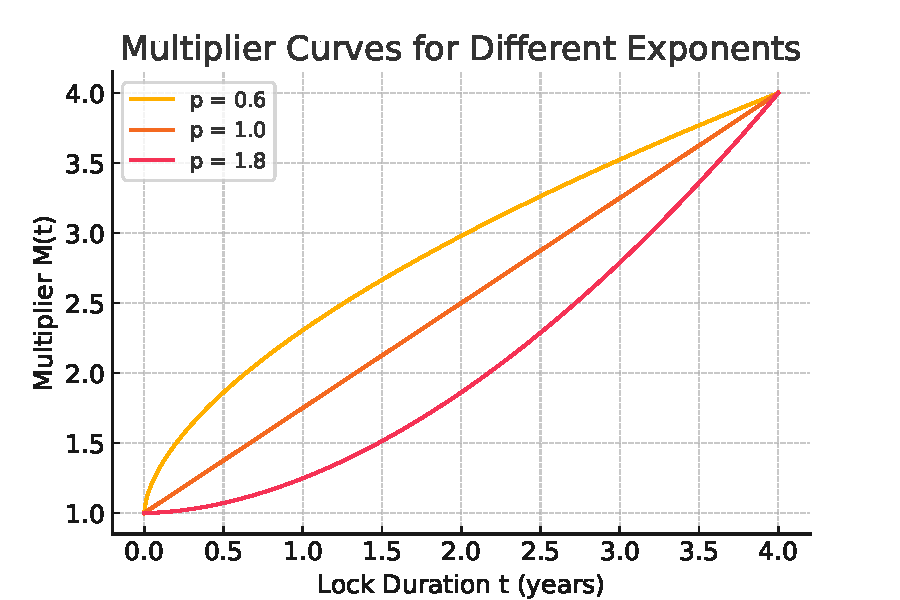
\includegraphics[width=0.65\textwidth]{curve_shapes.pdf}
\caption{Example multiplier curves for \(p=0.6,1,1.8\) under \(k=4\).}
\label{fig:curve}
\end{figure}

% ==================================================
\section{Minting and Lock Lifecycle}
Upon calling~\code{create\_lock}, a participant transfers~\(A\) tokens to an escrow vault. The runtime immediately computes
\begin{equation}
S = A\,M(t),
\label{eq:mint}
\end{equation}
and credits the account with~\(S\) synthetic governance tokens. These synthetic units remain outstanding until unlock, at which point they are burned atomically with the return of the base deposit.

% ==================================================
\section{Epochal Emission and Vesting}
At block heights divisible by the epoch length~\(\epsilon\) the chain mints a pool of new reward tokens, distributing them pro‑rata to synthetic balances~\(S\). Each beneficiary receives a vesting stream whose cumulative release follows the curve~\(V(d)\) for~\(0\le d\le t_{\text{vest}}\). Formally, a reward~\(R\) issued at \(d=0\) becomes liquid in amount~\(R\,V(d)\) after~\(d\) days. Governance may encode~\(V(\cdot)\) as:
\begin{itemize}
  \item A continuous function (e.g., exponential, hyperbolic) approximated with fixed‑point math, or
  \item A piecewise‑linear table~\(\{(d_i,v_i)\}_{i=0}^n\) interpolated on‑chain via monotone splines.
\end{itemize}
By default the system ships with a linear release~\(V(d)=d/t_{\text{vest}}\). Figure~\ref{fig:vesting} sketches several alternative shapes.
\begin{figure}[h]
\centering
\includegraphics[width=0.65\textwidth]{vesting_curve.pdf}
\caption{Sample vesting curves: linear, front‑loaded (\(V(d)=\sqrt{d/t_{\text{vest}}}\)) and cliff‑then‑linear. The \(y\)-axis shows the vested fraction; the \(x\)-axis counts days since issuance.}
\label{fig:vesting}
\end{figure}
The vesting buffer ensures that if arbitration later proves misconduct, any unvested slice~\(R\,[1-V(d)]\) can be confiscated.

% ==================================================
\section{Arbitration and Slashing Mechanics}
Validators supply attestations about off‑chain activity performed by agents or application modules. Either a multisig of trusted arbiters or a token‑weighted DAO can file an on‑chain \code{slash\_motion} referencing a specific validator, the contested epoch index and cryptographic evidence. Provided the motion is passed within the look‑back window~\(\lambda\), the runtime automatically removes the unvested fraction~\(R\,[1-V(d)]\) of each relevant reward stream and redirects the tokens to a community treasury. Optionally the motion may impose an additional penalty on the validator’s principal lock. Because unvested rewards are numerically linked to epoch identifiers, partial removal is a pure bookkeeping operation requiring no traversal of historical state.

% ==================================================
\section{Governance Flow in Continuous Prose}
The chain ships with a genesis configuration of \(k=4\), \(p=1\), \(\epsilon=43{,}200\)~blocks (approximately one week), \(t_{\text{vest}}=168\)~days (24 weeks) and \(\lambda=12\)~epochs. Token holders may later submit proposals to adjust any parameter or to upload an entirely new vesting table~\(V(\cdot)\). If the proposal passes the prescribed quorum and threshold, the runtime executes an automated call that updates the relevant storage items; existing locks and outstanding reward streams continue under their original parameters, whereas future emissions observe the revised curve. Emergency suspension of new locks is possible through a governance‑controlled switch that disables the public extrinsic while leaving unlocks unaffected.

% ==================================================
\section{Security Considerations}
Synthetic supply grants voting influence; therefore unduly generous multipliers or excessively front‑loaded vesting curves could threaten governance neutrality. The partial‑vesting plus retro‑slash construction mitigates short‑term bribery attacks by ensuring that ill‑gotten rewards remain claw‑back‑able until fully vested. All arithmetic employs 64‑bit fixed‑point saturating math to prevent overflow. To discourage griefing locks that bloat state, an early exit before the agreed term burns not only the synthetic balance but also a configurable share of the underlying principal.

% ==================================================
\section{Conclusion}
Time‑lock staking coupled with parametric multiplier and vesting curves aligns long‑term commitment with token issuance. By draping every emission in an arbitrarily shaped vesting veil that the DAO can slash retrospectively, the design reconciles capital efficiency with accountability. All numerical levers live in storage and may be tuned through standard governance motions, ensuring that economic policy evolves without disruptive code changes.

% ==================================================
\appendix
\section{Mathematical Proofs}
\label{app:proofs}
Proposition~1 establishes that~\(M(t)\) from Eq.~\eqref{eq:curve} is strictly increasing for any~\(k>1, p>0\). Differentiating yields~\(M'(t)=\frac{(k-1)p}{t_{\max}}(t/t_{\max})^{p-1}\), which is positive for~\(t>0\). Convexity follows by a second derivative argument:~\(M''(t)\ge0\) precisely when~\(p\ge1\). A bound on aggregate synthetic supply similarly derives from~\(M(t)\le k\), ensuring that~\(\sum S_i\le k\,A_{\text{lock}}\).

Proposition~2 shows that any monotone vesting curve~\(V(d)\) bounded by~\([0,1]\) preserves economic invariants: the sum of liquid plus unvested rewards never exceeds total emissions. Proof proceeds by induction on reward streams and leverages the fact that slashing only reduces outstanding balances.

\vspace{1em}
\textit{Further proofs, including a formal model of the vest‑slash game under rational adversaries and tight bounds on griefing costs, are under preparation and will accompany the audit report.}

\end{document}
